\documentclass[10pt,a4paper]{article}
\usepackage[latin1]{inputenc}
\usepackage{amsmath}
\usepackage{amsfonts}
\usepackage{amssymb}
\usepackage{graphicx}

\usepackage{blindtext}
\usepackage{scrextend}
\addtokomafont{labelinglabel}{\sffamily}
\title{Covariance and Sampling Code}
\begin{document}
\maketitle
\section{Introduction}

The sampling code is divided into two classes, \verb|Covariance| (Covariance.py), and \verb|Sampler|, (Sampler.py). The covariance object loads a power spectrum from a file, and computes value- and derivative- biased covariance matrices for the radial mode coefficients of the associated gaussian random field. These matrices are computed mode-by-mode (in the spherical harmonic decomposition), over a given radial grid. The same object then computes square-roots of these matrices, and can save and load the results of these computations to a .npz file. \verb|Covariance| is intended to be used to perform these computations, and then also to load and manage the resulting files. 

The second class, \verb|Sampler|, instantiates \verb|Covariance|, and uses it to access the roots of the covariance matrices. Sampler then generates random samples of the gaussian modes given a field height bias $\bar{\nu}$ and field number $N$. These modes are squared and summed pointwise to yield discrete samples of $\Phi_{00}(r)$, over the radial grid. Note that field height $\bar{\nu}$ and field number $N$ may be altered in the calls to \verb|Sampler|, without needing to recompute the covariance matrices. On the other hand, any changes to the power spectrum, its frequency domain, or the radial grid, will require recomputation of the covariance matrices and their roots.

This document will outline the structures of these classes (and will briefly discuss the classes which perform Levin integration), provide some comments and notes about their design, and specify issues that need to be resolved (minor issues, many of which have to do with interface). At the end, we'll present a comparison between the sample statistics generated by the code and the analytic statistics from the paper, and argue that these classes are behaving as expected.

\section{Covariance}
\subsection{Functions}

\begin{labeling}{covfuncs}
	\item [\textbf{\_\_init()\_\_}] The initializer doesn't take any arguments, but is rather used as a place to hard-code some parameters. In particular, the frequency-space resolution \verb|spectrum_spline_resolution| used to spline-fit the power spectrum and the factor by which to increase grid resolution when spline-fitting the correlations $\rho_C(r)$ and $\rho_D(r)$. \textbf{FIXME: should we also define a precision target here, or pass it to} \verb|ComputeCovariances()|?
	\item [\textbf{ComputeCovariances(fname\_spectrum, k\_low, k\_high, l\_max, r\_max, r\_step)}] This is the ``main'' function of the class. It calls all the other functions required to compute the covariance data in order. Argument \verb|fname_spectrum| is a filename for the power spectrum data, \verb|k_low| is the lower frequency cutoff to use when doing computations involving the power spectrum, \verb|k_high| is the corresponding upper cutoff frequency, \verb|l_max| is the maximum spherical harmonic $\ell$ mode to include, \verb|r_max| is the maximum radius in the grid (minimum is always at zero), and \verb|r_step| is the spacing between grid points. Note that both endpoints are included.
	The computation then takes place in steps,
	\begin{enumerate}
		\item Compute moments of the power spectrum
		\item Initialize the radial grid from \verb|r_max| and \verb|r_step|
		\item Fit splines to $\rho_C$ and $\rho_D$ over the appropriate radial domains with calls to \verb|ComputeRhoCSpline()| and \verb|ComputeRhoDSpline()|.
		\item Compute biased covariance matrices for each $\ell$ mode up to \verb|l_max| with call to \verb|ComputeCovarianceMatrices()|
		\item Compute a square root of the covariance matrix: a matrix $A$ such that $AA^T = \Sigma$, with call to \verb|ComputeSqrtCovariances()|.
	The covariance matrices and their square roots are stored as object member variables (See \verb|ComputeCovarianceMatrices()| and \verb|ComputeSqrtCovariances()|).
	\end{enumerate}

	\item[\textbf{LoadDummyPowerSpectrum()}] \textbf{FIXME: This is a testing function, to be replaced by LoadPowerSpectrum()}.
	Currently, this function fits a spline to the function $\exp(-k)$ over the region [\verb|k_low|, \verb|k_high|]. The fit is done with resolution \verb|self.spectrum_spline_resolution|, which is set in the constructor. Spectrum loaded to variable \verb|self.spectrum|.
	
	\item[\textbf{LoadPowerSpectrum()}] \textbf{FIXME: write this!} This will load
	the power spectrum from the file specified by \verb|self.fname_spectrum|, which is passed to \verb|ComputeCovariances()|.A spline will then be fit between \verb|k_low| and \verb|k_high| with \verb|self.spectrum_spline_resolution| points. \textbf{FIXME: maybe use k\_step instead, and pass as an argument to ComputeCovariances()?}.I'm waiting to see whether we use $k,\mathcal{P}(k)$ pairs, or $k,k^2\mathcal{P}(k)$ pairs to write this function, and to conform to the final choice of format for the spectrum file. Spectrum will be loaded to variable \verb|self.spectrum|.
	
	\item[\textbf{ComputeFrequencyCutoff(power\_fraction)}] This function computes an upper cutoff frequency $k_\mathrm{cut}$ based on the loaded power spectrum spline and a fraction $\alpha=$\verb|power_fraction| such that
	\begin{align}
		\int_{k_\mathrm{bottom}}^{k_\mathrm{cut}} \mathcal{P}(k)\, dk = \alpha 	\int_{k_\mathrm{bottom}}^{k_\mathrm{top}} \mathcal{P}(k)\, dk
	\end{align}
	This function is only here for convenience, and I'm guessing we may want to move its functionality earlier in the stack, so that the upper and lower bound frequencies in the spectrum file itself are already determined according to some reasonable physical criteria (like this one)
	\textbf{FIXME: note, this integral has as lower bound the lowest k available in the spline, not k\_low as passed to ComputeCovariances(). Also, k\_top is the highest value avaliable in the spline, and differs from k\_high.} Returns $k_\text{cut}$.
	
	\item[\textbf{ComputeSigmaN(n)}] This function computes the $n^\text{th}$ moment of the power spectrum according to Equation (7) in arXiv:1810.02078. Returns the moment.
	
	\item[\textbf{ComputeRhoC(r)}] Computes $\rho_C(r)$ as defined in Equation (82) of arXiv:1810.02078. Uses the Levin integration method \verb|ICalc| defined in the \verb|levin| module. Returns $\rho_C(r)$.
	
	\item[\textbf{ComputeRhoD(r)}] Computes $\rho_D(r)$ as defined in Equation (82) of arXiv:1810.02078. Uses the Levin integration method \verb|ICalc| defined in the \verb|levin| module. Returns $\rho_D(r)$.
	
	\item[\textbf{ComputeRhoCSpline()}] First computes a high-resolution discretization of $\rho_C$  over the range $[0,2r_\text{max}]$. The resolution is increased from the $r_\text{step}$ resolution by a factor of \verb|self.hires_factor|, which is set in the constructor. Fits a spline approximating $\rho_C$ to this discretization. The computation of the discretization is conditional on the corresponding variable having NoneType. Since this variable is saved in \verb|Save()|, this saves time if the array has been loaded. We save this array in addition to the covariance data because it is useful for computing analytics later on (for comparison to the samples). Spline stored at \verb|self.rho_c_spline|.
	
	\item[\textbf{ComputeRhoDSpline()}] Same as \verb|ComputeRhoCSpline()|, but for $\rho_D$, as defined in Equation (82) of arXiv:1810.02078, and over the range $[0,r_\text{max}]$. Spline stored at \verb|self.rho_d_spline|.
	
	\item[\textbf{ComputeRhoCLElement(l,r1,r2)}] Computes $\rho_{C_\ell}(r_1,r_2) = \tilde{C}_\ell(r_1,r_2)/\sigma_0^2$, where  $\tilde{C}_\ell$ is given in Equation (138) of arXiv:1810.02078. The integral in this definition is not badly oscillatory, and is done using the SciPy quad() routine. The integrand function evaluates the $\rho_C(r)$ spline, which is why we pre-compute it! Returns $\rho_{C_\ell}(r,r^\prime)$.
	
	\item[\textbf{ComputeCovarianceMatrices()}] Computes biased covariance matrix elements according to Equation (165) of arXiv:1810.02078. Calls \verb|ComputeRhoCLElement()| and evaluates the $\rho_C$ and $\rho_D$ splines in the process. The elements are stored in two different NumPy arrays, \verb|self.Covariances_leq1| and \verb|self.Covariances_lneq1|, depending on whether or not $\ell=1$ (which changes the biasing conditions). Each array has three indices. The first indicates which $\alpha$ field space component is being considered, which also alters the biasing conditions. The second and third indices are the radial grid indicies corresponding to the given covariance element.
	
	\item[\textbf{ScrubNegativeEigenvalues(eigvals)}] Takes a list of eigenvalues, \verb|eigvals|, and checks that all negative eigenvalues have absolute value $|\lambda|<1e-6$. Otherwise, throws an assertion. \textbf{FIXME: shouldn't hardcode this value. We may want to feed some kind of precision target to the Covariance object and base it off of that value.} If the negative eigenvalues are below this absolute value threshold, they are replaced by $0.0$. This compensates for negative eigenvalues arising from small numerical errors in the diagonalization of the covariance matrices performed in \verb|ComputeSqrtMatrix()|. Returns an array of scrubbed eigenvalues, \verb|clean_eigvals|.
	
	\item[\textbf{ComputeSqrtMatrix(mat)}] takes a 2D NumPy array \verb|mat| and computes matrices $M$ and $\Lambda$ (lambda diagonal) such that $M\Lambda M^T = \text{mat}$. Scrubs negative eigenvalues from $\Lambda$, and computes $A = M\sqrt{\Lambda}$, which satisfies $AA^T = \text{mat}$. Used by \verb|ComputeSqrtCovariances()|. Returns $A$.
	
	\item[\textbf{ComputeSqrtCovariances()}] Computes the $A$ matrices corresponding to each of the covariance matrices, making calls to \verb|ComputeSqrtMatrix()|. Stores the $A$ matrices in the same format as the covariance matrices, in variables \verb|self.sqrtcov_lneq1| and \verb|self.sqrtcov_leq1|.
	
	\item[\textbf{GetSqrtCovariance(l,alpha)}] A convenience function to simplify access to the $A$ matrices. Essentially just conditionals that take a pair $\ell,\alpha$ and return the root of the corresponding biased covariance matrix.
	
	\item[\textbf{Save(fname)}] Saves results from the calculations detailed above as NumPy arrays in a .npz file with filename specified by \verb|fname|.
	
	\item[\textbf{Load(fname)}] Loads results from the calculations detailed above from a NumPy array in a .npz file specified by \verb|fname|. Results are loaded to their corresponding object member variables, so if we pre-compute covariance data, then call \verb|Save()|, and then instantiate a new \verb|Covariance| object and call \verb|Load()|, the results of the computation can be accessed in the same way as in the original object. Some caveats: splines can't be saved to .npz files, and so must be re-computed from the discretizations. Also, the spectrum must be re-loaded if access to the spectrum is desired.
	\textbf{Note: for ``production'' usage, we will mainly just need to retrieve the $A$ matrices from the Covariance object, so we can just call Load() and then GetSqrtCovariance()}
\end{labeling}

\section{Levin}
I wont say too much about the Levin integration here (Levin.py), except to highlight the most important functions. There are two classes, \verb|LevinIntegrals|, which actually implements the levin method and the attendant collocation, and \verb|SphericalBesselIntegrator|, which implements an adaptive integration of ``I-type'' integrals. That is,
\begin{align} \label{eq:iint}
	I(\alpha) = \int_{a}^{b}dk\, f(k)j_\ell(\alpha*k).
\end{align}

\subsection{LevinIntegrals}
\begin{labeling}{levlabel}
	\item[\textbf{\_\_init\_\_(numpoints)}] Initialize variables for the computation. Most importantly, takes [numpoints] which is a positive integer determining the number of points to use in the collocation grid.
	
	\item[\textbf{compute\_I(a,b,alpha,l,func)}] Performs a levin integration of the I type integral determined by limits [a,b], 
	``radial parameter'' [alpha] (this will be the radius when we compute $\rho_C(r),\rho_D(r)$), spherical harmonic mode [l], and function [func] (which will be the power spectrum for our purposes). Returns the result of the integral.
\end{labeling}
\subsection{SphericalBesselIntegrator}
This class wraps the \verb|LevinIntegrals| function \verb|compute_I()| and provides case-checking and adaptive collocation resolution. 
\begin{labeling}{sphlabel}
	\item[\textbf{\_\_init\_\_()}] sets initial collocation resolution, as well as maximum recursion depth. Instantiates a LevinIntegrals object at the collocation resolution corresponding to each recursion level (resolution roughly doubles at each level). Also sets relative error tolerance. \textbf{FIXME: the relative tolerance should depend on some precision target we pass to our code at the beginning of our computations. We need to propagate this change here and elsewhere in the stack.}
	
	\item[\textbf{ICalc(a,b,alpha,l,func)}] Takes integration limits [a,b], radial coefficient [alpha], mode [l], and function [func] and computes the integral specified in Equation~\eqref{eq:iint}. First, we check whether $\alpha==0.0$ and $\ell=0$. If so, the integral reduces to an integral over the power spectrum (func), and we switch to quadrature. Otherwise, we begin with the two lowest-resolution LevinIntegrals objects, and perform the integrals. If their difference is below tolerance, we return the higher precision result. Otherwise, we recurse and take the next lowest resolution pair, and compare the difference to tolerance, and so on. Either we eventually suppress estimated error below tolerance, or hit the recursion limit. If the former, we return the result. If the latter, we make a last-ditch attempt with quadrature, and if that fails, throw an assertion.
	
	\textbf{Note: The non case-checked levin method fails when either $r$ or $\alpha$ is zero ($r\alpha$ appears in the argument to the spherical bessel function). The $\alpha=0$ case is handled in this function, but we get division by zero when the lower bound for k is zero. I think this never actually happens for real power spectra (the lowest k we feed into the covariance code is not zero), but we need to be aware of this!}
	
	\textbf{Note: There were originally two special cases in the levin code. First, $\alpha=0$ and $\ell=0$. This case reduces to an integral over the power spectrum, which is handled just fine. The second case (since removed) had some cutoff for $b$, the upper limit of momentum space. If $b$ were less than this cutoff, the code would resort to quadrature. I vaguely remember the levin method losing out to
	quadrature in the low-k regime (where the integrand does not oscillate), but I worried that this cutoff was arbitrary. 
	*update*: I did some preliminary checking against mathematica, and it doesn't seem to be the case that this outperforms levin in the stated regime (with an exponential dummy spectrum). So, I got rid of this second conditional. Note that the levin method will resort to quadrature anyway if the maximum number of collocation recursions is exceeded, so if the $b$ limit becomes a problem, and quadrature really is the way to go, the code should switch automatically.}
	
	\textbf{Note: The levin integration can take a long time for large $\alpha$ if we use a low resolution spline to fit the power spectrum (this showed up in testing against the exponential dummy spectrum). The moral of the story is that we should try upping spectrum resolution if the integrals are hanging.}
\end{labeling}

\section{Sampler}
This class is short and sweet. It simply extracts precomputed data from a Covariance object, carries out the gaussian sampling, and the subsequent construction of the $\Phi_{00}(r)$ sample.
\begin{labeling}{samplabel}
	\item[\textbf{\_\_init\_\_(covariance)}] Extracts some data from the
	Covariance object [covariance] and stores a copy as \verb|self.covariance|.
	
	\item[\textbf{GetSamples(nubar,nfields,nsamples)}] Takes a dimensionless field height [nubar], number of waterfall fields [nfields], and number of samples [nsamples], and returns a 2D array of biased samples of $\Phi_{00}$ over the radial grid specified in the Covariance object. The first index points to the sample number, and the second is the radial index within a given sample.
\end{labeling}
\section{Testing}

Ok, so I finally got around to doing a serious check of the covariance and sampling code!
I began with an exponential dummy spectrum,
\begin{align}
\mathcal{P}(k) = e^{-k},
\end{align}
where the lower and upper cutoffs for $k$ are given by $k_{lo} = 0.001$, $k_{hi} = 5.0$. 
Note: I need to implement the loading of the actual power spectrum. Will this be $\mathcal{P}(l)$ or $k^2\mathcal{P}(k)$? I'll need to alter the calculations accordingly.
First, I computed the mean of 1000 samples and compared the mean as a function of radius (together with standard error) to the analytic result for truncated $\ell$ given in Equation (184) of arXiv:1810.02078. The comparison is shown in Figure~\ref{fig:samplemean}. The errors are occluded by the markers, so i've zoomed in on the area with the worst discrepancy (highest variance) in Figure~\ref{fig:samplemeanzoom}. Even there, the agreement is quite good! Finally, I compared the sample variance of the 1000 samples to the analytic sample variance for truncated $\ell$ given in Equation (171), truncating $\ell$ at $\ell_\text{max}$ in the sums. This is shown (without standard error) in Figure~\ref{fig:samplevariance}.
\textbf{Note: I haven't yet implemented the ``add back'' of the droop in the sample mean. This should be pretty quick to do though.}
These test computations were done with the \verb|Test.py| script, which provides a simple implementation of the classes described here, and \verb|Analysis.py| which is essentially just doing the plotting.

	\begin{figure}
		\centering
		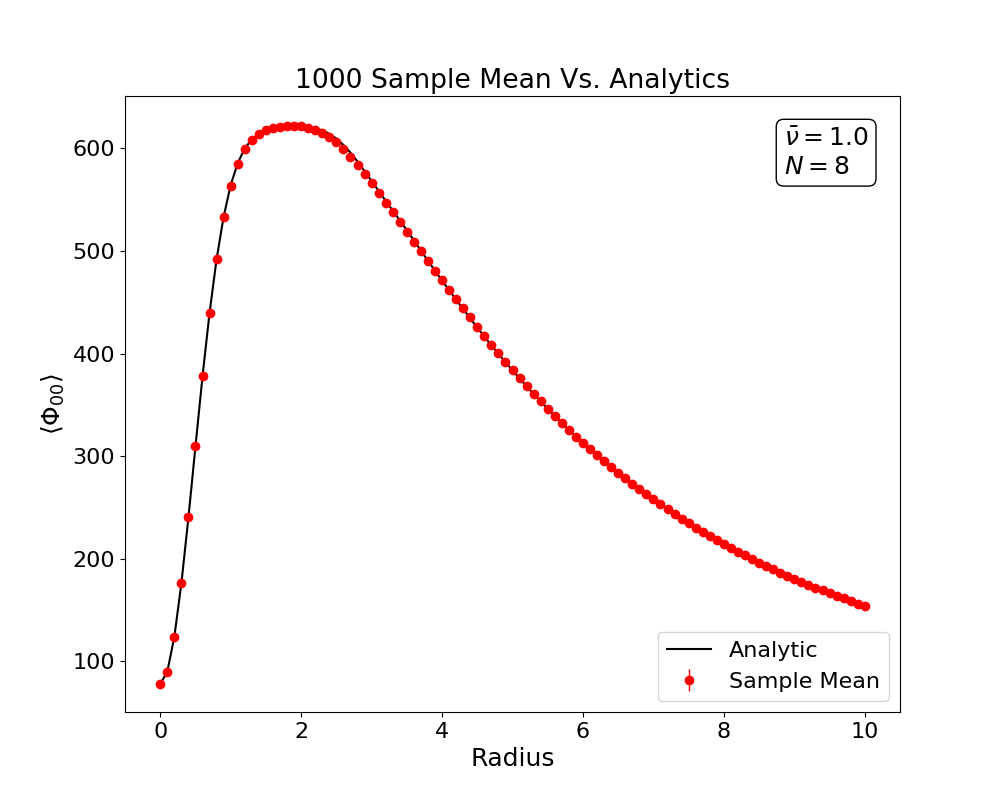
\includegraphics[width=0.9\linewidth]{/home/zander/physics/pbh/final_sampling_writeup/Images/sample_mean.png}
		\caption{}
		\label{fig:samplemean}
	\end{figure}
	\begin{figure}
		\centering
		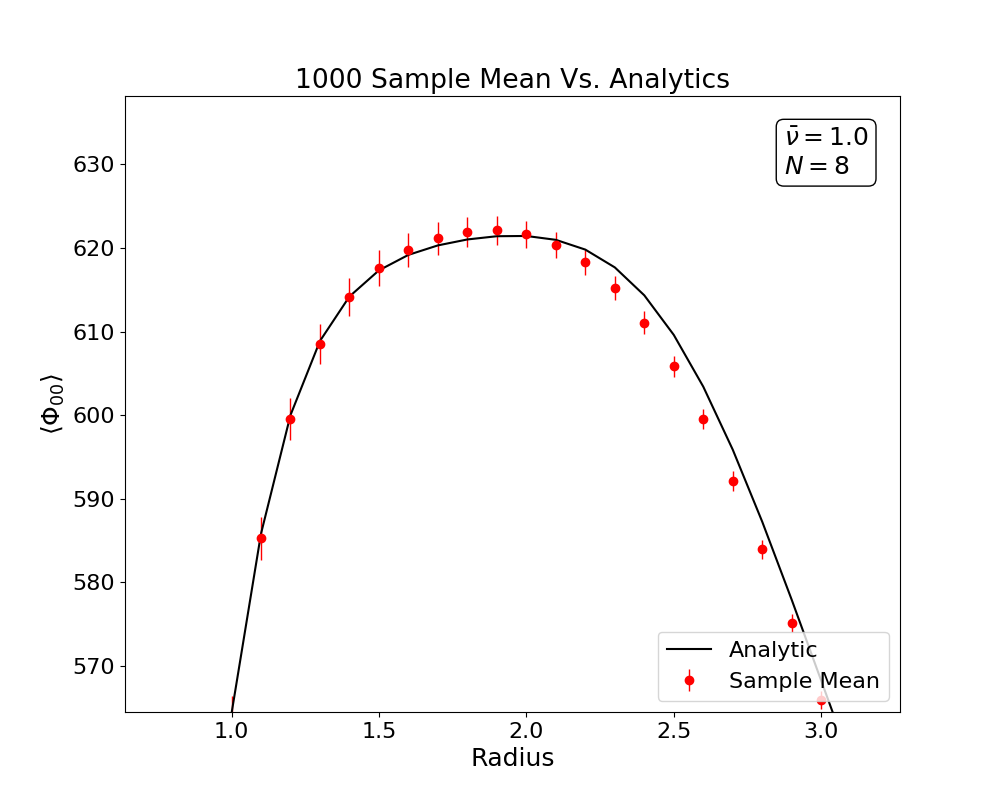
\includegraphics[width=0.9\linewidth]{/home/zander/physics/pbh/final_sampling_writeup/Images/sample_mean_zoom.png}
		\caption{}
		\label{fig:samplemeanzoom}
	\end{figure}
	\begin{figure}
		\centering
		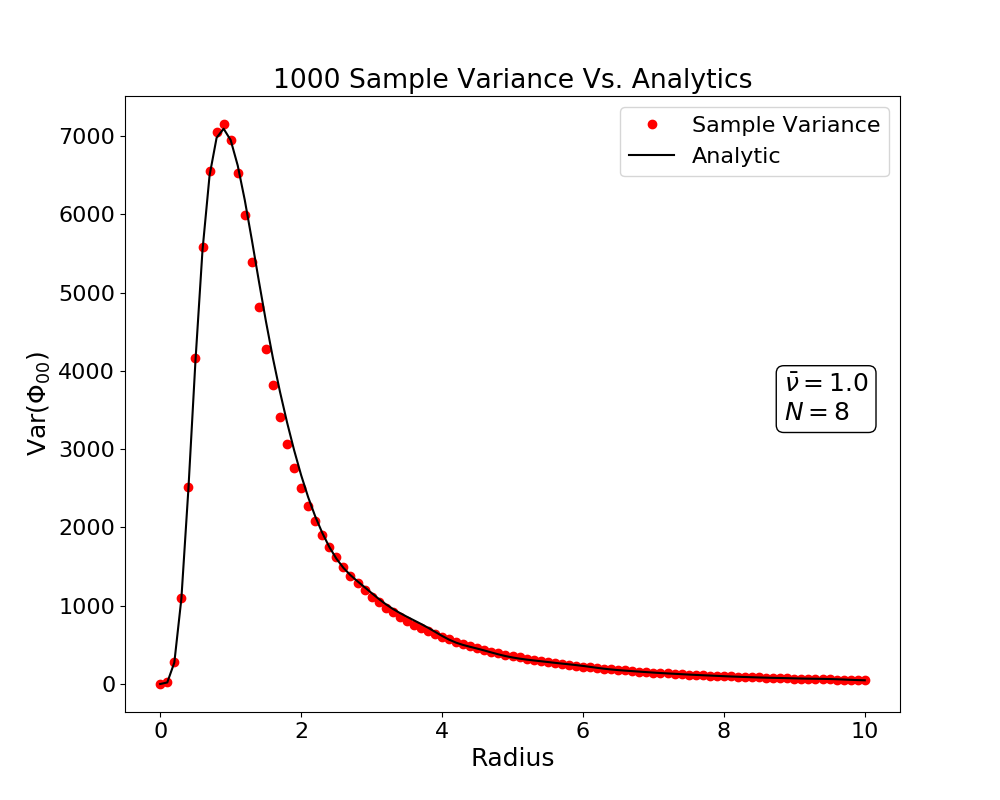
\includegraphics[width=0.9\linewidth]{/home/zander/physics/pbh/final_sampling_writeup/Images/sample_variance.png}
		\caption{}
		\label{fig:samplevariance}
	\end{figure}
	
\end{document}